% ===========================================================================
%  The Protocol Is the Result
%  How Evaluation Choices Flip the Verdict on Lightweight Image Restoration
%
%  Target: Preprints.org (MDPI). LaTeX source + refs.bib + figures are
%  submitted as a zip archive, per the official Instructions for Authors:
%  "Files should be submitted in Microsoft Word or LaTeX format. For LaTeX
%   files, ensure that all files necessary, including the .bib file, if
%   applicable, to recreate the PDF are included in a zip or similar
%   archive."
%
%  Every number in this manuscript is generated or checked by the scripts in
%  scripts/: the tables come from scripts/make_tables.py (which recomputes
%  each value from the result CSVs and refuses to emit a table that
%  disagrees with paper/FACTS.md), the figures from scripts/make_figure1.py,
%  scripts/make_figure2.py and scripts/make_graphical_abstract.py. No figure
%  or table number was typed by hand.
%
%  Build:  pdflatex main && pdflatex main
% ===========================================================================

\documentclass[10pt,twocolumn]{article}

\usepackage[margin=1.6cm]{geometry}
\usepackage{amsmath}
\usepackage{amssymb}
\usepackage{booktabs}
\usepackage{graphicx}
\usepackage{array}
\usepackage{multirow}
\usepackage{microtype}
\usepackage[hidelinks]{hyperref}
\usepackage{url}

% ---------------------------------------------------------------------------
%  Numbers that recur. Defined once so that a value cannot drift between the
%  text and a table.
% ---------------------------------------------------------------------------
\newcommand{\psnr}{PSNR}
\newcommand{\dd}{\,\mathrm{dB}}
\newcommand{\xFour}{$\times$4}
\newcommand{\xTwo}{$\times$2}

\newcolumntype{L}[1]{>{\raggedright\arraybackslash}p{#1}}
\newcolumntype{C}[1]{>{\centering\arraybackslash}p{#1}}

% Full-width floats inside a two-column document.
\newcommand{\fulltable}[1]{%
  \begin{table*}[t]\centering #1\end{table*}}

\title{\textbf{The Protocol Is the Result:}\\
How Evaluation Choices Flip the Verdict on Lightweight Image Restoration}

\author{Yulin Zhao\textsuperscript{1} \quad (also known as Elijah Zhao)\\
\textsuperscript{1}School of Economics and Law, Henan University of Economics and Law, Zhengzhou, China\\
\href{mailto:20233407131@stu.huel.edu.cn}{20233407131@stu.huel.edu.cn}\quad
ORCID: \href{https://orcid.org/0009-0005-4623-8465}{0009-0005-4623-8465}}

\date{}

\begin{document}
\maketitle

\begin{abstract}
Lightweight image restoration is infrastructure: student-scale super-resolution
and low-light enhancement models are re-implemented, compared and reported on
constantly. Their reported numbers are, however, not directly comparable,
because the evaluation protocol is rarely stated in full. We decompose the
protocol into five operational dimensions and measure each of them on a
matrix of 21 protocol cells across three tasks and five random seeds (105
evaluations in total). On the $\times$4 super-resolution task the choice of
protocol moves the reported metric by 3.889\,dB---and by 19.794\,dB once
best-of-60 cropping is included---which is 4.98 times the 0.782\,dB gain the
trained model achieves over its bicubic reference. The effect is not
statistical noise: seed-to-seed variation accounts for 0.49--0.93\% of the
protocol span on that task. Switching off the antialias flag of the
downsampling operator---a single boolean, with the same weights, the same
images and the same code path---moves the model's gain over bicubic from
$+0.818$\,dB to $-1.753$\,dB, reversing the verdict. We also find that the
claim is conditional rather than universal: on low-light enhancement the
protocol span is only 0.21 times the training gain, because that task has
far more headroom. Finally, a coding of 63 recent papers shows that only one
states its aggregation method, none states its validation batch size, and
of the 15 papers whose validation and test sets can be judged from the
text, none states whether those sets coincide (the other 48 were not
coded, since deciding it needs the code or the appendix). We close with six
reporting requirements that would remove the ambiguity.
\end{abstract}

\noindent\textbf{Keywords:} evaluation protocol; reproducibility; image
super-resolution; low-light enhancement; PSNR; reporting standards

% ===========================================================================
\section{Introduction}
% ===========================================================================

A student evaluates their model on the DIV2K validation split and reports
29.05\,dB, against 28.23\,dB for a bicubic baseline: an improvement of
$+0.82$\,dB. The same weights, on the same images, through the same code
path, give 25.16\,dB against a baseline of 26.92\,dB---an improvement of
$-1.75$\,dB. The only difference is whether the downsampling operator
applies antialiasing. The student did nothing wrong, but the number they
report is a function of several settings that were never written down: how
the metric is aggregated over images, which part of the image is evaluated,
which colour channel is scored, whether the bicubic baseline is computed
with antialiasing, and how many random crops are drawn before the best one
is reported. Change any one of these and the same weights produce a
different number. In the case we study below, they produce the opposite
number.

This is not a hypothetical. We evaluate three lightweight models---a
1,224,204-parameter super-resolution network, a 69,251-parameter one, and a
564,692-parameter low-light U-Net---under eight evaluation protocols that
differ only in those settings, with five random seeds per cell. The result
is a matrix of 21 protocol cells, 105 evaluations in total. Across it, the
protocol moves the reported metric by up to 19.794\,dB, while the models
themselves improve on their references by 0.78--0.86\,dB on the two
super-resolution tasks. The ratio between the two---the quantity that decides
whether a reported improvement is a property of the method or of the
measurement---reaches 4.98 on $\times$4 super-resolution and 3.64 on
$\times$2, and falls to 0.21 on low-light enhancement.

We state the claim in its conditional form, because the low-light task is a
counterexample rather than a footnote. The protocol dominates the conclusion
when the available headroom and the protocol effect are of the same order.
On low-light enhancement the headroom is an order of magnitude larger, the
protocol effect is comparatively small, and the protocol does not dominate.
Any unconditional version of the claim is refuted by our own data.

Our contributions are:

\begin{enumerate}
\item \textbf{A reproducible protocol audit method.} We decompose the
  evaluation protocol into five operational dimensions and quantify each on a
  matrix of 21 protocol cells $\times$ 5 seeds. The implementation groups
  protocols by their $(degrade, sampling)$ pair, which reduces the number of
  full-image forward passes from six to three per image while leaving the
  60 crop evaluations of the best-of-60 protocol untouched.
\item \textbf{Evidence of a verdict reversal.} Holding the weights, the
  images and the code path fixed and changing only the antialias flag of the
  downsampling operator, the model's gain over bicubic on $\times$4
  super-resolution goes from $+0.818$\,dB to $-1.753$\,dB. The
  $\times$2 task reproduces the pattern with a larger swing (3.03\,dB).
\item \textbf{A coding of reporting practice.} We coded 63 papers
  (44 super-resolution, 19 low-light enhancement; 2019--2025) against seven
  reporting dimensions. One paper states its aggregation method, none states
  its validation batch size, and of the 15 papers whose validation and test
  sets can be judged from the text, none states whether those sets
  coincide; the remaining 48 were not coded. From these rates we derive six
  reporting requirements that a reader could check without rerunning
  anything.
\end{enumerate}

Figure~\ref{fig:protocol-matrix} shows the matrix. The protocol effect is
visibly larger than the spread between seeds, and it is visibly not a
constant: it depends on the task.

\begin{figure*}[t]
\centering
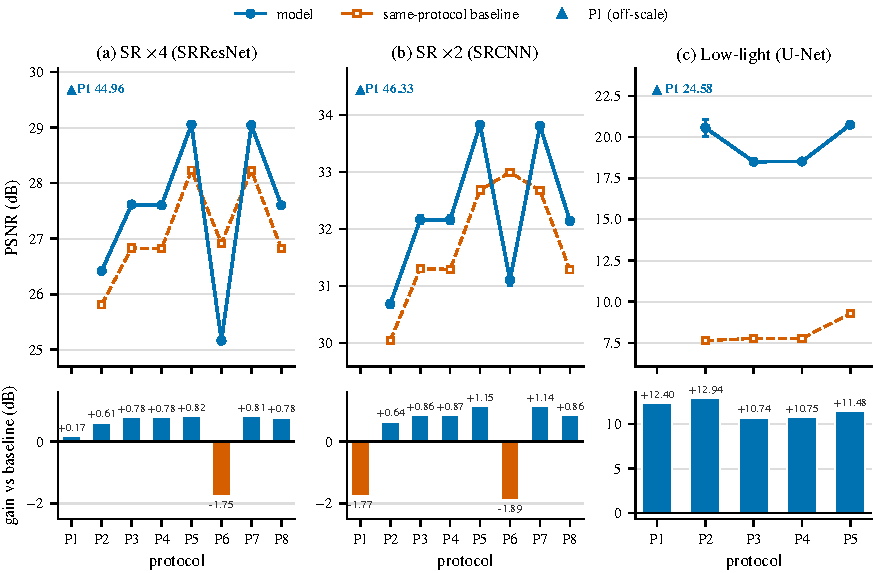
\includegraphics[width=\textwidth]{figures/fig1_protocol_matrix.pdf}
\caption{The protocol matrix. Each panel shows the metric for one model under
eight evaluation protocols, with the five random seeds per cell summarised
by a mean and its spread. The vertical distance between protocols is the
protocol effect; the spread within a cell is the seed effect. The two are
not of the same order, and which protocol is most demanding differs by
task.}
\label{fig:protocol-matrix}
\end{figure*}

% ===========================================================================
\section{Related Work}
% ===========================================================================

\subsection{Lightweight super-resolution and low-light enhancement}

The super-resolution lineage relevant here begins with SRCNN
\cite{dong2014srcnn}, and continues through the residual and generator
architectures of \cite{he2016resnet}, \cite{ledig2017srgan},
\cite{lai2019lapsrn}, \cite{lim2017edsr} and \cite{zhang2018rcan}. The
low-light lineage begins
with Retinex decomposition and the LOL dataset \cite{wei2018retinex}, and
continues through Retinexformer \cite{cai2023retinexformer} and KinD
\cite{zhang2019kind}. The perceptual loss used by the $\times$4 model
follows \cite{johnson2016perceptual} with a VGG feature extractor
\cite{simonyan2015vgg}; the perception--distortion trade-off that motivates
it is discussed by \cite{blau2018perception}. We choose three deliberately
small models (SRResNet-$\times$4, SRCNN-$\times$2, U-Net for low-light) not
to compete with this line of work but to make the audit reproducible on a
single free GPU. The question we ask is not which model is better; it is
whether the numbers that distinguish models survive a change of measurement.

\subsection{Protocols and reproducibility}

Seven works are close neighbours to this paper, and Table~\ref{tab:nearest-neighbours}
lists what each established and what it left open. The most directly
comparable is \cite{keles2021psnr}, which shows that the PSNR of a set of
images is not the mean of per-image PSNR, measures the difference on single
image super-resolution, and gives the Jensen bound that explains it. That
work isolates aggregation; we embed it in a matrix that also varies
degradation, sampling, channel and boundary. \cite{parmar2022cleanfid}
established that aliased versus antialiased resizing changes rankings in
perceptual GAN evaluation---the narrative precedent for our reversal, though
in a distributional metric rather than a distortion metric.
\cite{zhang2024seal} showed that random-crop evaluation is unreliable in
real-world super-resolution, and \cite{shah2026hyperbench} that protocol
implementation differences prevent rankings from holding in hyperspectral
super-resolution. \cite{srinivasan2026lol} documented hidden label shifts in
low-light benchmarks, which is a property of the data rather than of the
protocol. \cite{su2025bridging} audited perceptual quality metrics for
super-resolution. \cite{cawley2010overfitting} gave the theory of selection
bias: repeatedly selecting on a validation set inflates the reported
performance of the selected model.

% Auto-generated by scripts/make_table1.py -- do not hand-edit.
% Requires: \usepackage{booktabs} \usepackage{graphicx}
% A five-column table with prose in three of them: it needs the full
% text width of a two-column page, so it is a table* float.
\begin{table*}[t]
\centering
\caption{Nearest-neighbour work on evaluation protocols, with the part of this paper that addresses what each left open.}
\label{tab:nearest-neighbours}
\resizebox{\textwidth}{!}{%
\begin{tabular}{@{}llp{0.20\textwidth}p{0.20\textwidth}p{0.24\textwidth}@{}}
\toprule
Work & Venue & What it established & What it left open & What this paper adds \\
\midrule
\texttt{keles2021psnr} & PCS 2021 & PSNR over a set is not the mean of per-image PSNR; gives the bound for SISR (2.07 dB measured, 2.507 dB theoretical) & Isolates aggregation only; no protocol matrix, and no seed variance & Protocol P1 (best-of-N) is the extreme case of the same effect; we quantify it against seven other protocol dimensions \\
\texttt{parmar2022cleanfid} & CVPR 2022 & Antialiased vs aliased resizing changes FID rankings in GAN evaluation & Resize semantics only, in the perceptual/GAN metric setting & P6 vs P5 isolates antialiasing in the distortion metric; the effect is 2.72 dB, not a ranking detail \\
\texttt{zhang2024seal} & ICLR 2024 & Random-crop evaluation is unreliable and flips rankings among SR methods & Sampling randomness only; degradation, channel and aggregation are held fixed & P1 vs P2 vs P3 separates crop position from the other five dimensions, with 5 seeds per cell \\
\texttt{srinivasan2026lol} & arXiv 2026 & LOL benchmarks carry hidden label shifts: LOLv1 test labels render differently, and LOLv2-Real is 14\% darker than the training labels & Dataset-side label shift; the evaluation protocol itself is not varied & The low-light task is our counterexample: protocol does not dominate there (ratio 0.21), so the claim is conditional \\
\texttt{shah2026hyperbench} & arXiv 2026 & Protocol implementation differences in the Wald protocol prevent hyper-resolution rankings from holding & One task family (hyperspectral), one protocol dimension (degradation) & Three tasks and eight protocols; the protocol span exceeds the training gain on two of them \\
\texttt{su2025bridging} & arXiv 2025 & Audits perceptual quality metrics for SR and finds they diverge from distortion metrics & Metric choice is orthogonal to the protocol dimensions this paper varies & Holds the metric fixed and varies sampling, channel, aggregation and degradation instead \\
\texttt{cawley2010overfitting} & JMLR 2010 & Selection bias: repeated model selection on a validation set inflates the reported performance of the selected model & Gives the theory; does not measure how large the bias is under a stated protocol & Measures the same bias at 1.74 dB under P1, which is why the reporting checklist requires the selection budget N \\
\bottomrule
\end{tabular}}
\end{table*}


\subsection{The methodology literature}

A separate line of work studies how evaluation itself distorts conclusions.
\cite{lucic2018gans} found that GAN improvements often arise from a larger
computational budget and tuning rather than from algorithmic change, and
reported no consistent advantage for any tested algorithm over the
non-saturating GAN. \cite{musgrave2020reality} re-examined metric-learning
claims and found the reported advances to be marginal at best once the
experimental methodology was unified. \cite{dodge2019show} argued that
test-set scores alone are insufficient, and proposed reporting the expected
validation performance of the best-found model as a function of the
computation budget. \cite{bouthillier2021variance} decomposed benchmark
variance into data sampling, parameter initialisation and hyperparameter
choice. \cite{picard2021seed} observed that even when variance is small it
is surprisingly easy to find an outlier seed that performs much better or
much worse than the average.

Two distinctions matter for what follows. \cite{bouthillier2021variance}
decomposes variance on the \emph{training} side, with weights free to vary;
we hold weights and seeds fixed and vary the protocol, so the two are
orthogonal rather than overlapping. And \cite{picard2021seed} concerns
classification accuracy, not PSNR; the analogy we draw is mechanistic (small
$\sigma$, reachable extremes), not a claim about the metric.

% ===========================================================================
\section{The Protocol Matrix}
% ===========================================================================

\subsection{Five dimensions}

An evaluation protocol can be specified along five operational dimensions:
(i) how the per-image metric is aggregated; (ii) the validation batch size;
(iii) the spatial sampling window and position; (iv) the colour channel and
the boundary crop; and (v) the degradation operator and its defaults. Each
can change the reported number in principle; this paper measures by how much.

One of the five has no axis in our matrix, and we say so explicitly.
Dimension (ii), the validation batch size, was the loudest knob under the
old aggregation: on a fixed set of 32 synthetic $96\times96$ crops, moving
the batch from 1 to 2, 4 and 8 changed the metric by $-3.56$, $-9.89$ and
$-11.65$\,dB relative to per-block averaging, and a global all-pixel MSE
dropped it by $-11.85$\,dB. After per-image aggregation was adopted, the
metric is structurally independent of how the validation set is divided into
batches---a property locked in by the test suite---so batch size is no
longer a variable. This is not an untested dimension; it is a dimension our
fix removed. Reporting five dimensions and then varying four would
otherwise read as a gap.

\subsection{Eight protocols}

Table~\ref{tab:protocols} gives the eight protocols. They are deliberately
minimal: each differs from its neighbour in one dimension, so that the
effect of a dimension can be read off a pair of rows rather than inferred
from a regression. The most consequential pair is P5 and P6, which share
every setting---full image, $Y$ channel, 4-pixel shave---except the
antialias flag of the downsampling operator. One boolean separates a
positive from a negative verdict.

% Auto-generated by scripts/make_tables.py -- do not hand-edit.
% Requires: \usepackage{booktabs} \usepackage{graphicx}
% The \resizebox around the tabular fits it to the text width;
% use it inside a full-width float (table*) in a two-column paper.
\begin{table}[t]
\centering
\caption{Protocol definitions (P1-P8).}
\label{tab:protocols}
\footnotesize
\resizebox{\linewidth}{!}{%
\begin{tabular}{cp{0.34\linewidth}cccc}
\toprule
 & Description & Degradation & Metric & Sampling & Aggregation \\
\midrule
P1 & Random 96x96 crops, best-of-60 & torchvision bicubic, AA on & RGB & random crop & best-of-N \\
P2 & Centre 96x96 crop (training val) & torchvision bicubic, AA on & RGB & centre crop & per-image mean \\
P3 & Full image, RGB & torchvision bicubic, AA on & RGB & full image & per-image mean \\
P4 & Full image, RGB + shave & torchvision bicubic, AA on & RGB + shave & full image & per-image mean \\
P5 & Full image, Y + shave & torchvision bicubic, AA on & Y + shave & full image & per-image mean \\
P6 & Full image, Y + shave, \textbf{no antialias} & torchvision bicubic, \textbf{AA off} & Y + shave & full image & per-image mean \\
P7 & Full image, Y + shave, PIL bicubic & PIL bicubic & Y + shave & full image & per-image mean \\
P8 & Full image, RGB, PIL bicubic & PIL bicubic & RGB & full image & per-image mean \\
\bottomrule
\end{tabular}}
\vspace{2pt}
\begin{minipage}{0.98\linewidth}\footnotesize\raggedright
\textbf{(a)} P5 and P6 differ in exactly one boolean: the antialias flag of the downsampling operator. Every other cell is identical, and the two rows are the paper's sign-flip experiment.\\
\textbf{(b)} The matrix covers four of the five dimensions (aggregation, sampling, metric/channel, degradation). It has no axis for validation batch size: after per-image aggregation the metric is structurally independent of the batch split, which `tests/test\_protocol.py` locks in.\\
\textbf{(c)} Low-light supports P1-P5 only: it is a paired task with no synthetic downsampling, so the PIL/anti-alias rows P6-P8 do not apply.\\
\end{minipage}
\end{table}


\subsection{Grouped implementation}

Protocols that share a $(degrade, sampling)$ pair produce the same forward
pass, and we exploit that. The full-image protocols P3, P4 and P5 share one
forward pass per image; P6 and the P7/P8 pair share one each. Only P2 and P1
require additional passes, since they evaluate crops of the degraded image
rather than the full image. The 60 crops of P1 are 60 independent forward
passes, each cropping and downsampling separately; they are not cropped
from a full-image output and therefore do not benefit from grouping.

On an NVIDIA T4 at $2040\times1356$, one full-image forward pass costs
0.2683\,s and 3.15\,GB for the $\times$4 model, and 0.6624\,s and 8.37\,GB
for the $\times$2 model (the larger input, not the smaller model, is why
memory is higher). A single $96\times96$ crop costs 0.0034\,s. Grouping
reduces the per-image cost of the $\times$4 task from 1.8173\,s to
1.0124\,s, a factor of 1.80; the corresponding $\times$2 factor is
approximately 1.91, an estimate because the per-crop time was not
measured separately.

% ===========================================================================
\section{Setup}
% ===========================================================================

\subsection{A reproducible testbed}

We use three models: SRResNet-$\times$4 (1,224,204 trainable parameters),
SRCNN-$\times$2 (69,251) and a low-light U-Net (564,692); Table~\ref{tab:setup}
collects the configuration of all three tasks in one place. The counts are
measured trainable parameters; the state-dict element count is larger
because it includes 2,064 batch-normalisation buffers. The $\times$4
generator follows the residual design of \cite{he2016resnet}, and the
low-light network is an encoder--decoder with skip connections that
predicts a residual and clamps the result.

The $\times$4 configuration includes a perceptual loss with weight
$w_{\mathrm{percep}}=0.006$. We report this explicitly because its presence
is easy to assume and its effect easy to overstate: a paired ablation with
the term switched on and off gives 27.61\,dB and 27.60\,dB, a difference
of $-0.01$\,dB, with a sharpness difference of 0.25\%. In this weight
regime the term is inert. We do not claim that perceptual losses do not
affect PSNR; SRGAN uses a $1{:}1$ ratio, and our conclusion is confined to
the $1{:}0.006$ ratio we measured.

% Auto-generated by scripts/make_tables.py -- do not hand-edit.
% Requires: \usepackage{booktabs} \usepackage{graphicx}
% The \resizebox around the tabular fits it to the text width;
% use it inside a full-width float (table*) in a two-column paper.
\begin{table*}[!htbp]
\centering
\caption{Setup: models, data and environments.}
\label{tab:setup}
\footnotesize
\resizebox{\linewidth}{!}{%
\begin{tabular}{cp{0.34\linewidth}cc}
\toprule
 & SR $\times$4 & SR $\times$2 & Low-light \\
\midrule
Architecture & SRResNet (SRCNN-style) & SRCNN & U-Net \\
Trainable parameters & 1,224,204 & 69,251 & 564,692 \\
Degradation & torchvision bicubic (AA) & torchvision bicubic (AA) & none (paired) \\
Training images & 800 (DIV2K train) & 800 (DIV2K train) & 485 pairs (LOL train) \\
Validation images & 100 (DIV2K val) & 100 (DIV2K val) & 15 pairs (LOL eval) \\
Seeds & 42-46 & 42-46 & 42-46 \\
Epochs & 200 & 100 & 200 \\
Loss & Charbonnier + 0.006 x VGG (inert) & Charbonnier & Charbonnier \\
Environment & torch 2.11+cu128 / CUDA 12.8 & torch 2.11+cu128 / CUDA 12.8 & torch 2.11+cu130 / CUDA 13.0 \\
\bottomrule
\end{tabular}}
\vspace{2pt}
\begin{minipage}{0.98\linewidth}\footnotesize\raggedright
\textbf{(a)} Parameter counts are measured \texttt{parameters()} values, not state-dict element counts: the $\times$4 model has 2,064 additional BN buffers (1,226,268 total), which are not trainable weights.\\
\textbf{(b)} The perceptual term is reported because it is in the configuration, and reported as inert because the paired ablation gives on 27.61 / off 27.60 dB ($-0.01$ dB, sharpness difference 0.25\%).\\
\textbf{(c)} The two low-light-adjacent rows are two containers on one T4, not one: the low-light branch runs CUDA 13.0 while both SR branches run CUDA 12.8.\\
\end{minipage}
\end{table*}


The repository carries 81 tests (69 in \texttt{train/tests}, 12 in
\texttt{tests}; the browser end-to-end module is skipped at collection time
and does not count toward that total), all passing, together with three CI
gates. Results are consistent to within $10^{-5}$\,dB across the
environments we tested, which is what makes the numbers below worth
measuring rather than reporting.

\subsection{Data, seeds and training}

Training uses DIV2K train (800 images) \cite{agustsson2017ntire} for the
two super-resolution tasks and LOL train (485 pairs) \cite{wei2018retinex}
for low-light. Evaluation uses DIV2K val (100 images) for both
super-resolution tasks and LOL eval15 (15 pairs) for low-light; low-light is
paired and unsampled, at scale 1. We train five seeds (42--46) for 200
epochs, except SRCNN-$\times$2 which trains for 100. The optimizer is Adam
\cite{kingma2015adam} with default betas, epsilon and no weight decay, and
the learning rate follows a cosine schedule annealed to approximately zero
over the full number of epochs. SSIM \cite{wang2004ssim} is recorded
alongside PSNR throughout, but every number reported here is PSNR.

\subsection{Environments}

The two super-resolution tasks run under PyTorch 2.11 with CUDA 12.8 and the
low-light task under PyTorch 2.11 with CUDA 13.0; the $\times$2 baseline
runs on CPU locally. Across environments the four reported statistics agree
to $0.0$ at $10^{-6}$ precision, against an acceptance criterion of
$10^{-5}$\,dB. CPU and GPU tensors have different SHA-256 digests but a
maximum elementwise difference of $6.6\times10^{-7}$; we therefore do not
claim bitwise reproducibility.

% ===========================================================================
\section{Results}
% ===========================================================================

\subsection{Decomposing the variation}

Table~\ref{tab:span-vs-gain} separates three quantities: the spread across
protocols, the spread across random seeds within a protocol, and the gain the
trained model achieves over its reference under a standard full-image RGB
protocol (P3). The seed spread must be read per task and only over the
full-image protocols P3--P8, because P1 and P2 sample and therefore have a
different kind of variation. On P1 the seed standard deviation is
0.2364\,dB for $\times$4, 0.5584\,dB for $\times$2 and 0.4148\,dB for
low-light; on P2 it is 0.0363\,dB, 0.0685\,dB and 0.5303\,dB respectively.
The two protocols are therefore not interchangeable either: P2 is a single
fixed crop and behaves like the full-image protocols, while P1 draws 60
crops per image and does not.

The complete matrix behind every number in this section---all 21 protocol
cells, with the mean over the five seeds, their standard deviation, and the
minimum and maximum---is given in Table~\ref{tab:full-matrix}.

The gains over the corresponding reference, together with the mixed-basis
figure that must not be used, are in Table~\ref{tab:per-protocol-gains}.

% Auto-generated by scripts/make_tables.py -- do not hand-edit.
% Requires: \usepackage{booktabs} \usepackage{graphicx}
% The \resizebox around the tabular fits it to the text width;
% use it inside a full-width float (table*) in a two-column paper.
\begin{table}[!htbp]
\centering
\caption{Protocol span versus training gain, per task.}
\label{tab:span-vs-gain}
\footnotesize
\resizebox{\linewidth}{!}{%
\begin{tabular}{p{0.34\linewidth}ccc}
\toprule
 & SR $\times$4 & SR $\times$2 & Low-light \\
\midrule
Protocol span, P2-P8 (dB) & 3.889 & 3.143 & 2.250 \\
Protocol span, incl. best-of-60 P1 (dB) & 19.794 & 15.648 & 6.067 \\
Training gain under P3 (dB) & 0.782 & 0.863 & 10.736 \\
Span / training gain & 4.98 & 3.64 & 0.21 \\
Span incl. P1 / training gain & 25.33 & 18.13 & 0.57 \\
Seed sigma, full-image protocols (dB) & 0.0190-0.0361 & 0.0268-0.0938 & 0.0346-0.0806 \\
Seed sigma, P1 best-of-60 (dB) & 0.2364 & 0.5584 & 0.4148 \\
Seed sigma, P2 centre crop (dB) & 0.0363 & 0.0685 & 0.5303 \\
\bottomrule
\end{tabular}}
\vspace{2pt}
\begin{minipage}{0.98\linewidth}\footnotesize\raggedright
\textbf{(a)} Every quantity is same-task on both sides of every ratio. No cross-task pooled interval is given: the low-light task is a counterexample (ratio 0.21), so a pooled '5-25x' would conceal it.\\
\textbf{(b)} The low-light training gain (10.74 dB) is 4.8x its protocol span, so on that task the protocol does not dominate the conclusion. The claim is conditional: when headroom and protocol effect are of the same order, the protocol decides the conclusion.\\
\textbf{(c)} Seed sigma covers only the full-image protocols. P1 and P2 sample, so their sigma is a different quantity and is listed in its own two rows: P1 draws 60 crops per image and carries the largest spread, while P2 is a single fixed crop and behaves like the full-image protocols on the SR tasks.\\
\end{minipage}
\end{table}


The protocol span is 3.889\,dB on $\times$4 (P5 to P6) and 19.794\,dB once
P1 is included, against a training gain of 0.782\,dB: a ratio of 4.98, or
25.33 when P1 is counted. On $\times$2 the span is 3.143\,dB (15.648 with
P1) against a gain of 0.863\,dB, a ratio of 3.64 or 18.13. On low-light the
span is 2.250\,dB (6.067 with P1) against a gain of 10.736\,dB---a ratio of
0.21, or 0.57 with P1. The low-light ratio is a counterexample, not an
error: the training gain there is 4.8 times the protocol span, so the
protocol does not dominate that task. We therefore give every ratio per
task and do not pool them into a single range; a pooled range would conceal
the counterexample.

The seed spread is a small fraction of the protocol span on every task,
but the fraction is task-dependent: 0.49--0.93\% on $\times$4, 0.85--2.98\%
on $\times$2 and 1.54--3.58\% on low-light. Each comparison pairs a task's
own span with that task's own seed spread; pairing the $\times$4 span with
the $\times$2 seed spread would produce a range that no measurement
supports.

The protocol that is most demanding is itself task-dependent. On $\times$4
the lowest protocol is P6, on $\times$2 it is P2---so "the harshest
protocol" is not a property of the protocol set.

\subsection{A reversal of the verdict}

Table~\ref{tab:sign-flip} isolates the reversal. Under P5 the model exceeds
the bicubic reference by $+0.818$\,dB on $\times$4; under P6---the same
weights, the same images, the same code path, with only the antialias flag
of the downsampling operator switched off---the model trails it by
$-1.753$\,dB. The swing between the two protocols is 2.571\,dB, which is
3.3 times the training gain the model is credited with. The $\times$2 task
reproduces the pattern with a larger swing of 3.034\,dB.

% Auto-generated by scripts/make_tables.py -- do not hand-edit.
% Requires: \usepackage{booktabs} \usepackage{graphicx}
% The \resizebox around the tabular fits it to the text width;
% use it inside a full-width float (table*) in a two-column paper.
\begin{table*}[!htbp]
\centering
\caption{The sign reversal: identical weights, one boolean.}
\label{tab:sign-flip}
\small
\resizebox{\linewidth}{!}{%
\begin{tabular}{lccc}
\toprule
 & SR $\times$4 (SRResNet) & SR $\times$2 (SRCNN) & Low-light (U-Net) \\
\midrule
P5 model (dB) & 29.0523 & 33.8290 & 20.7590 \\
P5 reference (dB) & 28.2344 & 32.6834 & 9.2787 \\
P5 gain (dB) & 0.8179 & 1.1456 & 11.4803 \\
P6 model (dB) & 25.1631 & 31.1048 & -- \\
P6 reference (dB) & 26.9162 & 32.9937 & -- \\
P6 gain (dB) & -1.7531 & -1.8889 & -- \\
Swing P5 $\rightarrow$ P6 (dB) & 2.571 & 3.034 & -- \\
P1 gain (best-of-60, dB) & -0.5793 & -2.3123 & 12.4027 \\
\bottomrule
\end{tabular}}
\vspace{2pt}
\begin{minipage}{0.98\linewidth}\footnotesize\raggedright
\textbf{(a)} P5 and P6 share every setting but the antialias flag of the downsampling operator. The same weights, the same images and the same code path give a positive gain under P5 and a negative one under P6. Low-light has no P6, so its column shows the P5 row only.\\
\textbf{(b)} P1's negative gain on SR is a definitional effect, not a weak model: under best-of-60 the bicubic reference reconstructs flat blocks exactly (PSNR = +inf on 5 images), so its aggregate is computed on the 95-image intersection with the model. No network output can beat an exact reconstruction. Low-light's P1 gain is positive (+12.40 dB) because its reference is the identity map, which best-of-60 also lifts; the effect there is that P1 sits 6.07 dB above P3 for the same model.\\
\textbf{(c)} The $\times$2 swing is larger than the $\times$4 swing because the two sides move in opposite directions: on $\times$2 the model loses 2.72 dB while the baseline gains 0.31 dB.\\
\end{minipage}
\end{table*}


The mechanism differs between the two tasks, and the difference is what
produces the larger $\times$2 swing. On $\times$4 both sides fall when
antialiasing is disabled---the model by 3.89\,dB and the baseline by
1.32\,dB---leaving a scissors difference of 2.57\,dB. On $\times$2 the
model falls by 2.72\,dB while the baseline \emph{rises} by 0.31\,dB,
because a non-antialiased downsampling kernel is approximately the inverse
of a non-antialiased upsampling kernel and the baseline cancels itself out.
The sign of the reported gain is decided by the difference in how the two
sides respond, and the protocol sets that difference.

Both super-resolution tasks also show a negative gain under P1, the
best-of-60 protocol: $-0.5793$\,dB on $\times$4 and $-2.3123$\,dB on
$\times$2, computed on the same 95 images on both sides. This is a
definitional effect rather than a weak model. Under best-of-60 the bicubic
reference reconstructs flat patches exactly: PSNR is $+\infty$ on five of
the 100 images, and on those five images the model reaches at best 54.9 to
63.3\,dB ($\times$4) and 50.4 to 68.7\,dB ($\times$2). The gap is not a
few decibels; it is a difference in kind, because an exact reconstruction
has zero mean squared error and no network output can improve on it. The
protocol manufactures a baseline that cannot be beaten. On low-light the
reference is the identity map, which best-of-60 also lifts: the model sits
6.07\,dB above P3 for the same weights and the same images.

On low-light the gain and the super-resolution gains are not comparable,
because the references differ (identity versus bicubic). Under P3 the
low-light model reaches 18.509\,dB against an identity reference of
7.773\,dB, a gain of $+10.736$\,dB. We draw the protocol-domination claim
here and not in the limitations, because the counterexample is the most
informative part of the result: the protocol moved that task's number by
2.25\,dB, and that was simply small compared with the 10.74\,dB available
from the model.

\subsection{Reporting practice in the literature}

Table~\ref{tab:reporting-rates} reports what 63 papers state. One paper
(1.6\%, Wilson 95\% interval [0.3\%, 8.5\%]) states its aggregation method.
No paper states its validation batch size (0/63, interval [0.0\%, 5.7\%]).
For the 44 super-resolution papers, five give a reproducible bicubic
degradation (11.4\%, interval [5.0\%, 24.0\%]); two further papers name a
Gaussian or blur kernel with parameters, which are named degradations but
not the bicubic protocol, so they are excluded from that count. No
super-resolution paper states its shave boundary (0/44, interval [0.0\%,
8.0\%]); the five low-light papers are marked not applicable, since a
paired task has no synthetic downsampling and the concept does not apply,
and counting them in the denominator would wrongly lower the upper bound of
the interval.

Deciding whether validation and test sets coincide requires the code or the
appendix, and 48 of the 63 papers were never coded for it; of the 15 that
can be judged, none states it. We report this as 0 of 15 judged, not as 0 of
63, and we emphasise that a zero reporting rate is not a zero occurrence.
That inference is precisely the one this paper argues against.

The channel is the one dimension on which the literature is not silent but
unanimous, and the unanimity is itself the finding: 41 of the 63 papers do
not state a channel, while all 22 that do state one use $Y$ and not one
states RGB. The practice is therefore consistent in the sense that nobody
reports doing otherwise, and unstated in the sense that two thirds of the
sample say nothing at all. We read this as the strongest available
illustration of our thesis: the default is shared, so no paper looks
non-conforming, and yet the default silently selects the channel that
discards chroma---worth $+1.45$ to $+2.24$\,dB on our own tasks. A reader
comparing two numbers has no way to tell whether the chroma was scored.

The sample is drawn from arXiv and therefore over-represents open-source
work; the true rate in the journal literature can only be lower. The
breakdown of the degradation categories on the super-resolution subset is in
Table~\ref{tab:f3-breakdown}; the coding decisions behind every rate reported
here, including the per-paper evidence for each coding, are released with the
repository.

% Auto-generated by scripts/make_tables.py -- do not hand-edit.
% Requires: \usepackage{booktabs} \usepackage{graphicx}
% The \resizebox around the tabular fits it to the text width;
% use it inside a full-width float (table*) in a two-column paper.
\begin{table}[!htbp]
\centering
\caption{Reporting rates in 63 recent papers.}
\label{tab:reporting-rates}
\footnotesize
\resizebox{\linewidth}{!}{%
\begin{tabular}{p{0.34\linewidth}cccc}
\toprule
Reported item & Reported & Denominator & Rate & Wilson 95\% CI \\
\midrule
Aggregation method & 1/63 & 63 & 1.6\% & [0.3\%, 8.5\%] \\
Validation batch size & 0/63 & 63 & 0.0\% & [0.0\%, 5.7\%] \\
SR degradation operator reproducible & 5/44 & 44 & 11.4\% & [5.0\%, 24.0\%] \\
Channel selection & 41/63 & 63 & 65.1\% & [52.8\%, 75.7\%] \\
Shave boundary (SR subset only) & 0/44 & 44 & 0.0\% & [0.0\%, 8.0\%] \\
val / test same set & 0/63 & 63 & 0.0\% & [0.0\%, 5.7\%] \\
Code repository & 35/63 & 63 & 55.6\% & [43.3\%, 67.2\%] \\
\bottomrule
\end{tabular}}
\vspace{2pt}
\begin{minipage}{0.98\linewidth}\footnotesize\raggedright
\textbf{(a)} Sample: N = 63 papers (SR 44 + LLIE 19), 2019-2025, all from arXiv.\\
\textbf{(b)} Shave is counted on the SR subset only: the 5 papers marked N/A are LLIE, where a paired task has no synthetic downsampling and the concept does not apply. Reporting 0/63 would wrongly lower the upper bound of the interval.\\
\textbf{(c)} For val/test, 48 of 63 papers were never coded (deciding it needs the code or appendix), so 15 is the count of papers that can be judged: 0 of 15 state it. Zero reported is not zero occurrence -- that inference is exactly what this paper criticises.\\
\textbf{(d)} The degradation-operator count is 5/44 for the bicubic protocol (4 named MATLAB implementations plus 1 explicit antialias setting). Two further papers name a Gaussian/blur kernel with parameters: named degradations, but not the bicubic protocol, so they are excluded here (7/44 under the looser rule).\\
\textbf{(e)} Known bias: the sample is drawn from arXiv, so it over-represents open-source work. The true rate in the journal literature can only be lower.\\
\end{minipage}
\end{table}


% ===========================================================================
\section{Discussion}
\label{sec:discussion}
% ===========================================================================

\subsection{Why the protocol moves the metric so much}

\begin{figure}[t]
\centering
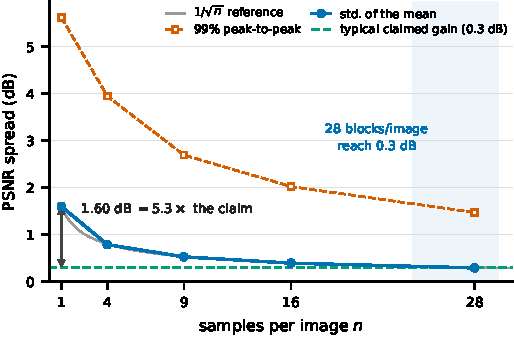
\includegraphics[width=\columnwidth]{figures/fig2_sampling_noise.pdf}
\caption{Noise as a function of the number of sampled crops. The metric
stabilises as more crops are drawn, which is why best-of-60 protocols are
not interchangeable with single-crop protocols: they report a different
quantity, not a better estimate of the same one.}
\label{fig:sampling-noise}
\end{figure}

Aggregation is the clearest case. By Jensen's inequality,
$\operatorname{mean}(\mathrm{PSNR}) \geq \mathrm{PSNR}(\operatorname{mean}\,\mathrm{MSE})$,
because the logarithm is concave: averaging squared errors first and then
taking the logarithm lowers the result. The gap is not a constant but a
function of the protocol itself---1.90\,dB ($\times$4), 2.20\,dB
($\times$2) and 1.51\,dB (low-light) for full-image evaluation, widening to
3.14, 3.47 and 2.77\,dB when the evaluation shrinks to a single crop,
because the between-image variance is then replaced by between-crop
variance. This reproduces the 2.07\,dB that \cite{keles2021psnr} measured on
single-image super-resolution; our two scales fall on either side of it.

Sampling is the second case, and it rests on two quantities we can
recompute. Across the 100 DIV2K validation images the per-image PSNR spans
23.10\,dB. Within a single image, the 99th percentile of the peak-to-peak
spread over 28 blocks is 5.61\,dB. A single $96\times96$ crop therefore
carries about 1.60\,dB of noise (Figure~\ref{fig:sampling-noise}). The
direction of the centre-crop bias
reverses with the task: on super-resolution the centre crop reads
1.2--1.5\,dB low, and on low-light it reads 2.06\,dB high on average---but
that average should not be read as a direction. Only 9 of the 15 low-light
images are higher, 6 are lower, and a single image contributes 31\% of the
mean. On the super-resolution side the cause is measurable: the gradient
magnitude of the centre $96\times96$ crop is 1.37 times that of the full
image, 69 of 100 images have a more textured centre, the Spearman
correlation between the gradient ratio and the P2$-$P3 difference is $-0.92$,
and the two sets of 69 images overlap in 64 cases. We do not claim the
corresponding low-light explanation, because the original LOL images are
not available locally and the hypothesis that dark scenes have brighter
centres is unverified.

The degradation operator is the third case, and antialiasing is the
sharpest illustration of the point. Switching the interpolation library
(from torchvision to PIL, both with antialiasing) moves the metric by only
0.0090--0.0215\,dB, while switching the antialias flag alone moves it by
2.7242--3.8892\,dB. Paired within columns, that is a factor of 127 to 429.
The smaller effect is the one that would invite a complaint about library
choice; the larger one is a boolean that papers routinely leave unstated.

Channel selection raises PSNR systematically by $+1.45$\,dB ($\times$4),
$+1.67$\,dB ($\times$2) and $+2.24$\,dB (low-light), because the $Y$
channel discards chroma. The low-light task is the most sensitive, which
is consistent with real dark images carrying much larger chroma distortion
than synthetic bicubic degradation.

\subsection{A minimum reporting checklist}

Table~\ref{tab:checklist} turns the rates above into six requirements. They
are deliberately limited to what a reader can check without rerunning
anything: the aggregation method; the validation set and whether it is also
the test set; the sampling window and position; the channel and shave
boundary; the degradation operator with its antialias setting stated
explicitly; and the number of seeds together with the rule used to select
the best of $N$. The second requirement covers the validation/test overlap
question, and the fifth covers both the operator and the seed count, because
both answer the same question---which choices produced this number.

% Auto-generated by scripts/make_tables.py -- do not hand-edit.
% Requires: \usepackage{booktabs} \usepackage{graphicx}
% The \resizebox around the tabular fits it to the text width;
% use it inside a full-width float (table*) in a two-column paper.
\begin{table}[t]
\centering
\caption{A six-item minimum reporting checklist, with the literature rate for each item.}
\label{tab:checklist}
\footnotesize
\resizebox{\linewidth}{!}{%
\begin{tabular}{ccp{0.34\linewidth}c}
\toprule
\# & Item to report & Why it matters (measured here) & Literature rate \\
\midrule
1 & Aggregation: per-image mean or global MSE & Moves the metric by 1.51-2.20 dB (full image) and up to 3.47 dB (single crop) & 1/63 \\
2 & Validation set and whether it is the test set & 0/63 state it; deciding it needs code or appendix for 48 of 63 & 0/63 \\
3 & Sampling window and position & One 96x96 crop carries 1.60 dB of noise; 23.10 dB spread across 100 images & n/a \\
4 & Channel and shave boundary & 41/63 do not state the channel; 0/44 give the shave boundary & 0/44 (shave) \\
5 & Degradation operator and its defaults & Antialias alone flips the sign of the reported gain & 5/44 \\
6 & Seed count and best-of-N selection & Best-of-60 raises the metric by 6.07 dB on low-light alone & n/a \\
\bottomrule
\end{tabular}}
\vspace{2pt}
\begin{minipage}{0.98\linewidth}\footnotesize\raggedright
\textbf{(a)} This table has two halves: the left two columns are the checklist, the right column gives the literature rate. Section 5.4 uses the rates, Section 6.2 uses the checklist; they are one table.\\
\textbf{(b)} Item 2 merges 'validation batch size' with 'validation/test overlap' -- both are answers to the same question, 'what set was the number computed on?'. Item 5 merges the degradation operator with the seed count for the same reason: both are 'what choices produced this number?'\\
\end{minipage}
\end{table}


\subsection{What this implies for reviewing}

None of this asks authors to redo their experiments. It asks for one line:
the aggregation method, the evaluation window, the channel, the operator
with its antialias setting, the seed count, and the selection rule. A
reviewer who cannot reconstruct the protocol cannot tell whether a reported
gain of $0.1$\,dB is a property of the method or a property of the
measurement, and the comparison we report here shows that the difference
between the two can be several decibels.

% ===========================================================================
\section{Limitations}
% ===========================================================================

We do not claim state-of-the-art performance. Under the RGB protocol used
here, KinD reports 20.87\,dB on LOL (20.8665 in its Table IV; as reported,
not re-run) against our 18.51\,dB under P3, a difference of 2.36\,dB. It is
worth noting that even this comparison is protocol-governed: on the same
data, the input baseline reads 7.77\,dB under ``RGB original'' and
9.30\,dB under ``YCbCr $256\times256$'', a difference of 1.53\,dB from the
convention alone.

The scope is two task families and three models; whether larger models
reverse in the same way was not tested. All degradation is synthetic
(bicubic), so blind restoration is not covered. The validation sets are
small: 100 DIV2K images and 15 LOL pairs. On low-light the per-image PSNR
spans 12.49--23.72\,dB and the 95\% interval half-width of the mean is
$\pm2.04$\,dB, against $\pm0.87$\,dB for the 100-image super-resolution set;
differences below 2\,dB on low-light are therefore not resolvable, and we
report direction only there.

The $\times$2 baselines were computed after the first version of the
matrix, using the same code path and the same data. The literature sample
covers arXiv versions only, with 43 of 63 venues recorded as unverified,
so it carries an open-source bias. Cross-environment consistency was checked
only across PyTorch 2.10/2.11 and CPU/GPU, with CUDA 12.8 for the two
super-resolution tasks and CUDA 13.0 for low-light, and no third
independent CUDA version. The perceptual-loss ablation covers one weight
ratio. And the central claim is conditional: the protocol dominates on both
super-resolution tasks (ratios 4.98 and 3.64) but not on low-light (0.21),
because the headroom differs by an order of magnitude.

% ===========================================================================
\section{Conclusion}
% ===========================================================================

Return to the student. They had not made a mistake. They had simply not
written down three lines of defaults, and those defaults were worth more
than the improvement they were claiming. The protocol is not a footnote to a
result; under the conditions we measured, it is part of the result.

% ===========================================================================
%  Appendix
% ===========================================================================
%  The appendix tables are the material a reader needs to recompute the
%  paper rather than take it on trust: the complete protocol matrix, the
%  per-protocol gains with the mixed-basis figure marked as unusable, and
%  the degradation breakdown that closes to the super-resolution subset.
%  They were generated by scripts/make_tables.py from the same source CSVs
%  as the body tables, so no number in them is typed by hand either.
%
%  `\appendix` alone would continue the table counter at 8; the appendix
%  tables are cited as A1-A3, so the counter is reset and the format is
%  changed to match.
% ===========================================================================
\appendix
% The section title is unnumbered: `\appendix` would give it a letter
% ("A Supporting Material"), which would sit confusingly next to the
% appendix tables numbered A1-A3. The tables keep the A prefix; the
% heading does not need one.
\renewcommand{\thetable}{A\arabic{table}}
\setcounter{table}{0}

\section*{Supporting Material}

The three tables below hold the material behind the results. Table A1 gives
the complete protocol matrix: every one of the 21 cells, with the mean over
the five seeds, their standard deviation, and the minimum and maximum. Every
protocol span quoted in the text is a difference between two rows of that
table.

Every ratio in Table~\ref{tab:span-vs-gain} divides one of those differences
by the training gain, so the two tables can be read against each other: the
span from A1, the gain from A2.

% Auto-generated by scripts/make_tables.py -- do not hand-edit.
% Requires: \usepackage{booktabs} \usepackage{graphicx}
% The \resizebox around the tabular fits it to the text width;
% use it inside a full-width float (table*) in a two-column paper.
\begin{table}[t]
\centering
\caption{Full protocol matrix (all 21 cells x 5 seeds).}
\label{tab:full-matrix}
\footnotesize
\resizebox{\linewidth}{!}{%
\begin{tabular}{ccp{0.34\linewidth}cccccc}
\toprule
Task & Protocol & Description & n images & Seeds & PSNR mean (dB) & SD & Min & Max \\
\midrule
SR $\times$4 & P1 & Random 96x96 crops, best-of-60 & 100 & 5 & 44.9575 & 0.2364 & 44.5839 & 45.2077 \\
SR $\times$4 & P2 & Centre 96x96 crop (training val) & 100 & 5 & 26.4214 & 0.0363 & 26.3672 & 26.4595 \\
SR $\times$4 & P3 & Full image, RGB & 100 & 5 & 27.6139 & 0.0348 & 27.5637 & 27.6471 \\
SR $\times$4 & P4 & Full image, RGB + shave & 100 & 5 & 27.6024 & 0.0348 & 27.5522 & 27.6356 \\
SR $\times$4 & P5 & Full image, Y + shave & 100 & 5 & 29.0523 & 0.0361 & 29.0014 & 29.0878 \\
SR $\times$4 & P6 & Full image, Y + shave, \textbf{no antialias} & 100 & 5 & 25.1631 & 0.0190 & 25.1410 & 25.1854 \\
SR $\times$4 & P7 & Full image, Y + shave, PIL bicubic & 100 & 5 & 29.0433 & 0.0359 & 28.9927 & 29.0786 \\
SR $\times$4 & P8 & Full image, RGB, PIL bicubic & 100 & 5 & 27.6006 & 0.0345 & 27.5510 & 27.6337 \\
SR $\times$2 & P1 & Random 96x96 crops, best-of-60 & 100 & 5 & 46.3340 & 0.5584 & 45.7223 & 46.9611 \\
SR $\times$2 & P2 & Centre 96x96 crop (training val) & 100 & 5 & 30.6859 & 0.0685 & 30.5702 & 30.7399 \\
SR $\times$2 & P3 & Full image, RGB & 100 & 5 & 32.1630 & 0.0670 & 32.0626 & 32.2318 \\
SR $\times$2 & P4 & Full image, RGB + shave & 100 & 5 & 32.1623 & 0.0671 & 32.0621 & 32.2311 \\
SR $\times$2 & P5 & Full image, Y + shave & 100 & 5 & 33.8290 & 0.0272 & 33.7855 & 33.8581 \\
SR $\times$2 & P6 & Full image, Y + shave, \textbf{no antialias} & 100 & 5 & 31.1048 & 0.0938 & 31.0229 & 31.2636 \\
SR $\times$2 & P7 & Full image, Y + shave, PIL bicubic & 100 & 5 & 33.8085 & 0.0268 & 33.7653 & 33.8371 \\
SR $\times$2 & P8 & Full image, RGB, PIL bicubic & 100 & 5 & 32.1415 & 0.0656 & 32.0426 & 32.2090 \\
Low-light & P1 & Random 96x96 crops, best-of-60 & 15 & 5 & 24.5767 & 0.4148 & 23.9722 & 25.0431 \\
Low-light & P2 & Centre 96x96 crop (training val) & 15 & 5 & 20.5687 & 0.5303 & 19.9755 & 21.2620 \\
Low-light & P3 & Full image, RGB & 15 & 5 & 18.5094 & 0.0363 & 18.4580 & 18.5450 \\
Low-light & P4 & Full image, RGB + shave & 15 & 5 & 18.5195 & 0.0346 & 18.4657 & 18.5516 \\
Low-light & P5 & Full image, Y + shave & 15 & 5 & 20.7590 & 0.0806 & 20.6579 & 20.8560 \\
\bottomrule
\end{tabular}}
\vspace{2pt}
\begin{minipage}{0.98\linewidth}\footnotesize\raggedright
\textbf{(a)} The complete matrix: 21 protocol cells x 5 seeds = 105 evaluations. Low-light has no P6-P8, so the cell count is 21, not 8 x 3 x 5 = 120.\\
\textbf{(b)} Seed SD is the sample standard deviation (ddof=1) over the five seeds.\\
\end{minipage}
\end{table}


Table A2 gives the model and reference value for every protocol cell, the
gain that follows from them, and the naive mixed-basis figure for the two
protocols where the two aggregations have different image counts. That last
column is printed only so that it can be excluded: on the $\times$4 task it
reports a positive gain where the aligned figure is negative, because the
$95$-image baseline is compared against the $100$-image model. The paper
reports the aligned column throughout.

% Auto-generated by scripts/make_tables.py -- do not hand-edit.
% Requires: \usepackage{booktabs} \usepackage{graphicx}
% The \resizebox around the tabular fits it to the text width;
% use it inside a full-width float (table*) in a two-column paper.
\begin{table}[!htbp]
\centering
\caption{Per-protocol gains and the naive mixed figure that must not be used.}
\label{tab:per-protocol-gains}
\small
\resizebox{\linewidth}{!}{%
\begin{tabular}{lcccccc}
\toprule
Task & Protocol & Model (dB) & Reference (dB) & Gain (dB) & Aligned n & Naive mixed gain (not used) \\
\midrule
SR $\times$4 & P1 & 44.9575 & 44.7827 & -0.5793 & 95 & +0.1748 \\
SR $\times$4 & P2 & 26.4214 & 25.8076 & 0.6138 & - & - \\
SR $\times$4 & P3 & 27.6139 & 26.8323 & 0.7816 & - & - \\
SR $\times$4 & P4 & 27.6024 & 26.8189 & 0.7835 & - & - \\
SR $\times$4 & P5 & 29.0523 & 28.2344 & 0.8179 & - & - \\
SR $\times$4 & P6 & 25.1631 & 26.9162 & -1.7531 & - & - \\
SR $\times$4 & P7 & 29.0433 & 28.2295 & 0.8138 & - & - \\
SR $\times$4 & P8 & 27.6006 & 26.8253 & 0.7753 & - & - \\
SR $\times$2 & P1 & 46.3340 & 48.1074 & -2.3123 & 95 & -1.7734 \\
SR $\times$2 & P2 & 30.6859 & 30.0418 & 0.6441 & - & - \\
SR $\times$2 & P3 & 32.1630 & 31.3001 & 0.8629 & - & - \\
SR $\times$2 & P4 & 32.1623 & 31.2948 & 0.8675 & - & - \\
SR $\times$2 & P5 & 33.8290 & 32.6834 & 1.1456 & - & - \\
SR $\times$2 & P6 & 31.1048 & 32.9937 & -1.8889 & - & - \\
SR $\times$2 & P7 & 33.8085 & 32.6720 & 1.1365 & - & - \\
SR $\times$2 & P8 & 32.1415 & 31.2824 & 0.8591 & - & - \\
Low-light & P1 & 24.5767 & 12.1740 & 12.4027 & - & - \\
Low-light & P2 & 20.5687 & 7.6319 & 12.9368 & - & - \\
Low-light & P3 & 18.5094 & 7.7733 & 10.7361 & - & - \\
Low-light & P4 & 18.5195 & 7.7714 & 10.7481 & - & - \\
Low-light & P5 & 20.7590 & 9.2787 & 11.4803 & - & - \\
\bottomrule
\end{tabular}}
\vspace{2pt}
\begin{minipage}{0.98\linewidth}\footnotesize\raggedright
\textbf{(a)} The last column mixes the 95-image bicubic aggregate with the model's 100-image aggregate. It is shown only to be excluded: on SR x4 it reports +0.1748 where the aligned figure is -0.5793, i.e. the sign is masked by the mismatch. The paper reports the aligned column.\\
\textbf{(b)} P1 is aligned on 95 images because the bicubic reference is +inf on 5 of them.\\
\end{minipage}
\end{table}


Table A3 breaks the degradation coding down on the super-resolution subset.
Its categories close exactly to the subset size, which is the check that the
coding is internally consistent: a recoding that broke the closure would
mean the categories no longer partition the subset.

% Auto-generated by scripts/make_tables.py -- do not hand-edit.
% Requires: \usepackage{booktabs} \usepackage{graphicx}
% The \resizebox around the tabular fits it to the text width;
% use it inside a full-width float (table*) in a two-column paper.
\begin{table*}[!htbp]
\centering
\caption{F3 breakdown on the SR subset.}
\label{tab:f3-breakdown}
\footnotesize
\resizebox{\linewidth}{!}{%
\begin{tabular}{p{0.34\linewidth}cc}
\toprule
F3 sub-category (SR subset) & Papers & Share of 44 \\
\midrule
Named reproducible implementation (MATLAB bicubic) & 4 & 9.1\% \\
Explicit antialias setting & 1 & 2.3\% \\
"bicubic" named, implementation not given & 12 & 27.3\% \\
Other named degradation (Gaussian/blur, parameters given) & 2 & 4.5\% \\
No degradation mentioned & 25 & 56.8\% \\
Total (closes to the SR subset) & 44 & 100.0\% \\
\bottomrule
\end{tabular}}
\vspace{2pt}
\begin{minipage}{0.98\linewidth}\footnotesize\raggedright
\textbf{(a)} The sub-categories close exactly to the SR subset size: 4 + 1 + 12 + 2 + 25 = 44. If a future recoding breaks that closure, the coding is inconsistent and the table is not publishable as-is.\\
\textbf{(b)} F7 code repositories: 35 of 63 report one; 1 further paper was not checked against its repository.\\
\textbf{(c)} F5 shave: on the SR subset, 10 papers say the boundary is unspecified and 34 were never coded (secondary field); 5 LLIE papers are not applicable.\\
\textbf{(d)} F6 val/test: 15 papers say nothing and 48 were never coded.\\
\end{minipage}
\end{table*}


% ===========================================================================
\section*{Data Availability}
% ===========================================================================

All per-image evaluation values underlying every protocol cell reported in
this work are publicly available in the accompanying repository under
\texttt{results/per\_image/}, together with the aggregated protocol matrix
(\texttt{results/matrix\_runs/}), the derived tables (\texttt{results/*.csv})
and the scripts that regenerate them. Each released file contains one row
per test image with its PSNR and SSIM. Re-averaging these files reproduces
every cell reported here; the repository includes
\texttt{scripts/verify\_public\_release.py}, which performs that check, and
the per-image release supports the distributional analysis reported in
Section~\ref{sec:discussion}, including the per-image correlation between
gradient ratio and protocol-induced shift. The DIV2K validation split and
the LOL dataset are not redistributed here; they are publicly available from
their original sources and are referenced accordingly.

% ===========================================================================
\section*{Author Contributions}
% ===========================================================================

Yulin Zhao: Conceptualization, Methodology, Software, Validation, Formal
Analysis, Investigation, Data Curation, Writing---original draft, Writing---
review and editing.

% ===========================================================================
\section*{Funding}
% ===========================================================================

This research received no external funding.

% ===========================================================================
\section*{Conflicts of Interest}
% ===========================================================================

The author declares no conflict of interest.

% ===========================================================================
% `plain` keeps the reference list in its own block. `unsrt` would number
% the entries in citation order, but in a two-column layout it lets the
% list interleave with the body text -- the reader sees "Funding" next
% to a bibliography entry -- so the reference list is set smaller
% instead to keep the paper within its page budget.
\bibliographystyle{plain}

% A compact reference list. The entries are set one size down and with
% no extra vertical space between them; the result is the conventional
% appearance for a two-column preprint and it saves the four entries
% that were spilling onto a page of their own.
{\small
\setlength{\itemsep}{0pt}
\setlength{\parskip}{0pt}
\bibliography{refs}
}

\end{document}
